\documentclass[a4paper,12pt]{article}
\usepackage[utf8]{inputenc}

\usepackage[UKenglish]{babel}
\usepackage[babel]{csquotes}

\usepackage{amsmath, amssymb}
\usepackage{graphicx, subcaption, booktabs}

\usepackage[colorlinks=true, allcolors=blue]{hyperref}
\usepackage[all]{hypcap}

\usepackage[style=authoryear, backend=biber, natbib]{biblatex}
\bibliography{~/Zotero/Bibliothek.bib}

\usepackage{setspace}
\doublespacing


%opening
\title{How to reduce Item Nonresponse in Face-to-Face Surveys? A Review and Evidence from the European Social Survey}
%\author{Malte Grönemann \\ University of Mannheim, Mannheim, Germany}

\begin{document}

\maketitle

\begin{abstract}
I review the literature on item nonresponse in surveys. Based on this review, I extend the satisficing model with respondents' privacy concerns to incorporate all relevant aspects of the response process for item nonresponse. I review proposed strategies to reduce item nonresponse and test selected strategies. Results suggest that boosting respondents' use of showcards and interviewing in the respondents' primary language might be promising ways to reduce item nonresponse. Other people present during the interview have only a small association with the number of refusals. Matching the age and gender of respondents and interviewers appears not to be a worthwhile strategy.
\end{abstract}

Keywords: item nonresponse, survey design, survey error, face-to-face surveys, fixed-effects negative binomial regression

\section{Introduction}

Missing data pose a problem to the analysis of survey data. They decrease the effective sample size and can introduce bias to estimates if the causes for missingness are related to the item or respondent characteristics \citep{deleeuwPreventionTreatmentItem2003}. Although missing data are rare in most single items, they can add up to a considerable loss of observations in multivariate analyses. Item nonresponse can also be seen as an indicator of overall data quality since it can result from \textit{satisficing} \citep{krosnickResponseStrategiesCoping1991}. Satisficing means that the respondent is giving a satisfactory answer instead of the best one. Due to these harmful effects of missing data, one objective of survey researchers is to keep their prevalence as low as possible. Therefore, it is important to understand the processes that can lead to missing data.

I review the existing literature on item nonresponse and extend the satisficing model based on this review to include privacy concerns resulting in an encompassing model of item nonresponse: the probability of item nonresponse depends on the task difficulty of the item(s) divided by the product of ability and motivation of the respondent or the respondents' privacy concerns. This means that higher difficulty results in more item nonresponse and higher ability and motivation in less item nonresponse. Difficulty, ability, and motivation are separate from privacy concerns, e.g. due to item sensitivity or general mistrust. Privacy concerns are relevant when deciding whether to disclose information and do not influence the cognitive burden of retrieving the answer.

I then turn to practical strategies that could be used to decrease item nonresponse by reviewing proposed strategies. In the empirical part of the paper, I compare the effects of selected strategies. Promoting the use of showcards and translating questionnaires appear to be most promising. Both of those reduce the cognitive burden of respondents. Matching respondents' and interviewers' gender and age does not reduce item nonresponse. They could have influenced item nonresponse if respondents are more willing to share private information with interviewers similar to themselves. The results are not causal though. However, the results indicate that strategies aiming at a lower cognitive burden for respondents are our best guess to improve data quality.

This introduction follows a short theoretical discussion presenting a theoretical model for the probability of item nonresponse based on satisficing. Structured by this model, I review the literature on strategies how to reduce item nonresponse and test a selection using the \textit{European Social Survey}. The rest of the paper is devoted to this test of strategies, describing data and methods and presenting results. Finally, I summarise and discuss my review and results.


\section{A Model of Item Nonresponse}

Whether respondents answer a survey question and which answer they give is always a cognitive process taking place at the very moment of the interview. The \textit{survey response process} \citep{tourangeauPsychologySurveyResponse2000} involves multiple steps on behalf of the respondent. They need to comprehend the question, retrieve information from memory, eventually judge this information, map them onto the response options, and perhaps edit the response due to sensitivity or social desirability. Respondents will most likely take these steps in order but they can jump back and forth, e.g. if they need to form an opinion on the spot. But in all of these steps, item nonresponse can be introduced \citep{deleeuwPreventionTreatmentItem2003}.

The two types of item nonresponse, "Don't know" and refusal, might be related to different steps of the survey response process though. Refusals are likely introduced in the editing step when respondents do not want to answer a question although they could. They may find certain information to be too sensitive or they may not feel comfortable sharing it with the interviewer due to a lack of trust. DK is likely as an answer when the respondent cannot give a substantive answer. Either the respondent cannot answer because they do not know about the content of the question or are unable to remember an event \citep{beattyAnswerNotAnwer2002, turnerCanResponseLatencies2015}. In this situation, DK is a valid response and does not constitute a problem for data quality.
On the other hand, they might not see value in putting in the effort to give an optimal response and \textit{satisfice} \citep{krosnickResponseStrategiesCoping1991}. Satisficing refers to various shortcuts (heuristics) that survey respondents can take when answering questions. One of these shortcuts is item nonresponse. The data collected in this case are of lower quality.

However, \citet{shoemakerItemNonresponseDistinguishing2002}  have
shown that higher mental effort is related to more refusals as well. And
conversely, it is plausible that DK is used as a more polite way to refuse.
In the following sections, I will therefore not distinguish between refusal and DK even though they may have varying strengths of predictors \citep{silberEffectsQuestionRespondent2021}. Similarly, I will not consider the unproblematic case of DK as a genuine answer although differentiating between the two meanings of DK might be relevant for substantive analyses.

In the continuation of this section, I will discuss theoretical concepts that impact the likelihood of item nonresponse in the cognitive process of response formation. Later, I will combine these concepts into a theoretical model based on satisficing \citep{krosnickResponseStrategiesCoping1991}.

When it comes to item nonresponse, the key concept is the \textit{ability} of the respondents to carry out cognitive tasks. Differences in cognitive abilities are the main explanation for differences in item nonresponse across education, age, and health \citep{colsherDataQualityAge1989, pickeryImpactRespondentInterviewer1998, deleeuwPreventionTreatmentItem2003, messerDeterminantsItemNonresponse2012, silberEffectsQuestionRespondent2021}. Ethnic minorities tend to have a higher rate of item nonresponse likely caused by lower literacy and worse command of the majority language \citep{kupekDeterminantsItemNonresponse1998, pickeryImpactRespondentInterviewer1998}. \citet{meitingerPowerCultureItem2020} conclude that item nonresponse reflects broader social inequalities in abilities and access to information. The ability hypothesis is directly supported by correlations between item nonresponse and measures of intelligence \citep{hedengrenDogThatDidn2012}.

The second relevant concept is \textit{task difficulty}. When questions are more difficult or unclear, they tend to have higher rates of nonresponse \citep{holbrookImpactQuestionRespondent2006, messerDeterminantsItemNonresponse2012, holbrookInterviewerErrorsHelp2016, olsonEffectsRespondentQuestion2019}. Demographic questions are usually easier for respondents to remember, resulting in lower rates of item nonresponse compared to attitudinal and behavioral questions, which may require respondents to formulate an answer on the spot \citep{olsonEffectsRespondentQuestion2019, silberEffectsQuestionRespondent2021}.

Even if people can complete a task, they may not want to do it unless they feel that the effort is worthwhile. They need to have the \textit{motivation} to provide an optimal response. That explains why people who are more interested in the topic of a survey are less likely to leave items unanswered \citep{kochItemNonresponseEuropean2009, silberEffectsQuestionRespondent2021}. Item nonresponse is linked to conscientiousness measures as well \citep{hedengrenDogThatDidn2012}.

The editing process can also be influenced by motivation. For instance, respondents and interviewers may choose not to answer screening and filtering questions on purpose to lessen the survey workload \citep{tourangeauMotivatedMisreportingShaping2015}. This statement pertains only to data collections where the respondents know or can guess which questions serve as filters though.

When editing an answer, respondents may have concerns about their \textit{privacy}\footnote{ I use this label to encompass overall privacy concerns related to the survey, such as data processing and anonymity, as well as the desire to avoid answering specific sensitive questions}. Will the interviewer judge me if I answer truthfully? Can I trust that my data will be kept secure and confidential? This is a particular problem for questions perceived as intrusive \citep{tourangeauSensitiveQuestionsSurveys2007} like questions on income \citep{yanTrendsIncomeNonresponse2010} and sexual behaviour \citep{kupekDeterminantsItemNonresponse1998}, which often show particularly high levels of item nonresponse. However, when it comes to attitude questions about controversial political issues such as immigration, there tends to be more item nonresponse as well \citep{piekutSurveyNonresponseAttitudes2021}. Item nonresponse is indeed frequently used as a measure of question sensitivity \citep{tourangeauSensitiveQuestionsSurveys2007}. Respondents will likely have such privacy concerns immediately when they hear a sensitive question and jump from the comprehension stage to the editing stage in the survey response process \citep{tourangeauPsychologySurveyResponse2000}. They probably refuse to answer before an honest answer has been formed.  Increased item nonresponse is associated with reluctance and skepticism towards surveys and science, general privacy concerns, and mistrust \citep{silberEffectsQuestionRespondent2021}. 

\bigskip

Based on the reviewed literature, I have identified four concepts that affect the probability of item nonresponse in surveys: cognitive ability, task difficulty, motivation, and privacy concerns. However, as \citet{krosnickResponseStrategiesCoping1991} already hypothesised, these concepts are interrelated in their effect on item nonresponse. Very easy questions can be answered by less able respondents and very hard questions might even cause the most able to struggle. The resulting fraction of difficulty by ability represents the relative mental effort to answer a question. And a highly motivated respondent answers even difficult questions. \citet[225]{krosnickResponseStrategiesCoping1991} formalised the probability of satisficing. 

Item nonresponse is such a satisficing strategy. Additionally, higher privacy concerns lead to more item nonresponse as well. Since this relates to another step in the survey response process, namely editing rather than comprehension, retrieval or judging, I postulate it to be independent from the other concepts. 

For a complete theoretical model of harmful item nonresponse, privacy concerns therefore need to be added to the model by \citet{krosnickResponseStrategiesCoping1991}. As these concepts are (partially) interrelated and have a nonlinear relationship to item nonresponse, it is useful to formalize and summarize their relationship as follows:

$$ P_{INR} \ = f\left(\ max \left( \frac{difficulty}{ability \ * \ motivation} \ , \ privacy \right)\right) $$

\textit{The probability of an ingenuine nonsubstantive answer on behalf of the respondent is a function of the task difficulty divided by the ability and motivation of the respondent or the respondents' privacy concerns, whichever is higher.}

Please note that this theoretical model is not able to and not intended to predict the probability of item nonresponse in a given item, as highlighted by the fact that it is an undefined function. Therefore, the individual concepts do not require measurement. The maximum function emphasizes that there are two independent mechanisms, and only the dominant one will impact item nonresponse at a time. This theoretical model specifically addresses item nonresponse for a single item but its meaning is adaptable to every level of a survey.


\section{How to reduce Item Nonresponse}

With these four concepts in mind, we can develop strategies to reduce item nonresponse and ensure better data quality in our surveys. Some of the following strategies may seem obvious and are already established standards in survey design not only because of their potential relationship to item nonresponse but to ensure the quality of substantial answers as well. Others might reduce item nonresponse but they could have negative consequences for other parts of total survey error, the combined effect of all error sources in a survey \citep{grovesTotalSurveyError2010}. They require a trade-off before implementation.

I have structured this review of strategies to reduce item nonresponse by the respective concepts they target.

\subsection{Task Difficulty}

The level of difficulty of a task is largely determined by how the questions are designed and what type of answer is expected. To make tasks easier, it is recommended to ask short, straightforward questions that avoid any confusion or unclear concepts. Asking respondents to complete multiple tasks at once should also be avoided. For a more thorough guide on how to design questions and questionnaires, see e.g. \citet{smythDesigningQuestionsQuestionnaires2016}. The difficulty of a task is related to the type of question as well. Questions that are open-ended or allow for multiple options and ordering of categories are more likely to result in higher nonresponse rates than closed single choice items \citep{schumanOpenClosedQuestion1979, holbrookImpactQuestionRespondent2006, holbrookInterviewerErrorsHelp2016, olsonEffectsRespondentQuestion2019, silberEffectsQuestionRespondent2021}. To make it easier for respondents, visual aids like images or showcards can be used. Showcards eliminate the need for respondents to recall all response categories while answering a question. However, there is limited research on how showcards affect item nonresponse. According to a study by \citet{holbrookInterviewerErrorsHelp2016}, using showcards in survey questions led to more unanswered items. However, this may have been because showcards were only used for more challenging questions. In the European Social Survey (ESS), showcards do not appear to impact the distribution of meaningful responses in survey experiments, as noted by \citep{jackleAssessingEffectData2010}, although they did not investigate item nonresponse.

How question design affects levels of item nonresponse is very well understood and differences between questions constitute the largest part of the variance in item nonresponse \citep{olsonEffectsRespondentQuestion2019}. This highlights the importance of the single question for overall data quality.

It is important to design the entire questionnaire as simply as possible, not just the individual questions. Questionnaires that include changes in response scales, routing, and filtering tend to result in higher rates of nonresponse \citep{messerDeterminantsItemNonresponse2012}. However, routing and filtering should not increase difficulty in computer-assisted modes. Grouping questions by topic could reduce the required mental effort and item nonresponse but it also increases the likelihood of non-differentiation between items \citep{krosnickResponseStrategiesCoping1991}. Explicitly offering DK and refusal options can increase their use, as it makes respondents more aware of the possibility of an "easy way out" \citep{schumanAssessmentNoOpinion1979, beattyAnswerNotAnwer2002}.

To reduce task difficulty for members of language minorities, the questionnaire can be translated so that respondents can take the interview in the language they are most proficient in. But translating questionnaires can be costly and may affect the comparability of cases. For a review on comparability in cross-cultural surveys, see e.g. \citet{behrTranslationMeasurementInstruments2016}.

To enhance the quality of survey design, identify any errors, and ensure that respondents can complete the required tasks, it is recommended to thoroughly review the questionnaire and its implementation for data collection. Common methods for doing so include conducting reviews and pilot studies.

\subsection{Ability}

While we cannot alter the general cognitive ability of our respondents, we can influence their ability to answer survey questions at the time of participation. To ensure a productive interview, it is important to choose an environment that encourages focus and clear communication. If possible, opt for quiet and not distracting locations at appropriate times. Having other people present during an interview can be distracting, but there is no conclusive evidence to support this claim \citep{kupekDeterminantsItemNonresponse1998, tuSocialDistanceRespondent2007, silberEffectsQuestionRespondent2021}. Respondents may become fatigued during lengthy interviews \citep{holbrookInterviewerErrorsHelp2016, olsonEffectsRespondentQuestion2019}.

\subsection{Motivation}

Motivation could decrease throughout the interview as well. While web surveys have used different page layouts and progress bars to combat this issue, the effectiveness of these methods is uncertain \citep{peytchevWebSurveyDesign2006, yanShouldStayShould2011, sarrafSurveyPageLength2014}. The research on cooperation enhancement, such as through incentives, has mainly focused on unit nonresponse. However, some of these methods could also be effective in increasing item nonresponse. After all, unit and item nonresponse are linked: respondents that initially refused to participate have higher levels of item nonresponse \citep{yanRelationUnitNonresponse2010, frickerExaminingRelationshipNonresponse2010}.

\subsection{Privacy Concerns}

Survey researchers should address privacy concerns to encourage respondents to answer by ensuring the security and anonymity of their data. It is important to communicate why the data is collected, how it will be processed, and how privacy is protected. This is not only ethically advisable but also often a legal requirement.

When conducting face-to-face surveys, the trust between the respondent and interviewer is influenced by their relationship. Scholars have hypothesized that respondents are more likely to trust interviewers who they perceive to be similar to themselves. To test this hypothesis, studies have been conducted to examine the impact of matching characteristics between the respondent and interviewer. \citet{vercruyssenEffectSociodemographicMis2017} observe less item nonresponse when interviewers and respondents are matched in age. Additionally, matching gender reduces item nonresponse for males but increases it for females. \citet{piekutSurveyNonresponseAttitudes2021} found female interviewers experienced higher rates of nonresponse but there was no significant correlation between the gender of the interviewer and the gender of the respondent. \citet{silberEffectsQuestionRespondent2021} found that education matching has no effect while \citet{tuSocialDistanceRespondent2007} find age and education matching to be potent predictors of item nonresponse. A test that could be interesting to conduct is whether pairing interviewers and respondents who share the same immigration status and/or ethnicity would make a difference. Immigrants tend to have higher levels of item nonresponse, language barriers, and I could imagine that some of them may be mistrustful towards interviewers due to racist experiences and a fear of discrimination.

\section{Strategies to be Tested}

So far, this article has reviewed and summarized the literature on item nonresponse in surveys. I have suggested a theoretical model, an extension of the satisficing model by \citet{krosnickResponseStrategiesCoping1991}, as a conceptual summary that can inform our survey design and I have reviewed strategies to reduce item nonresponse and categorized them accordingly. In the remainder of the article, I am going to test a few selected strategies to reduce item nonresponse derived from the theoretical model and the literature review. All of these strategies could change at least one of the four concepts from the theoretical model and therefore could have a causal connection to item nonresponse. Whether these strategies actually do change the associated concepts and how strongly their effect translates into changes in item nonresponse will be central to my empirical analysis.

\begin{enumerate}
 \item During an interview, respondents may experience a decrease in concentration and motivation to answer questions as time goes on. As a result, item nonresponse may become more common the longer the interview lasts. To maintain high data quality and reduce item nonresponse, it might be advisable to keep questionnaires as short as possible.

 \item It is likely that interferences and the presence of others during an interview can cause item nonresponse, as they may distract the respondent and make them hesitant to answer certain questions in front of people they know. As a result, it might be beneficial that interviews are conducted without other people present, if feasible.

 \item To make answering easier for respondents, showcards could be provided so they do not have to remember the response scale. Showcards would then lower the required cognitive effort and reduce item nonresponse.

 \item Respondents who primarily speak a different language at home may face difficulties in the response process. To ensure data quality from these respondents, one option is to translate the questionnaire, although this can be costly and may present comparability problems.

 \item According to previous studies, people may feel more comfortable answering questions from interviewers who share similar social characteristics, such as gender and age. If true, survey agencies could assign interviewers based on demographic information if it is available in the sampling frame.
\end{enumerate}

Table 1 summarises the selected strategies that I am going to test in my empirical analysis. The second column shows which concepts play a role in the hypothesized mechanism linking the respective strategy to item nonresponse. The third column gives the expected direction of the relationship between strategy and item nonresponse, e.g. the longer the questionnaire, the more item nonresponse. These are also the expected signs of the coefficients if the strategies work as imagined.

\begin{table}[h]
\caption{Reduction Strategies to be Tested}
\centering
\begin{tabular}{| l l l |}
\hline
Strategy & Mechanism & Expectation \\
\hline
Length of the Questionnaire & Ability, Motivation & positive \\
Interference of the Interview & Ability, Privacy & positive \\
Use of Showcards & Difficulty & negative \\
Interview not primary Language & Difficulty & positive \\
Gender Matching & Privacy & negative \\
Interviewer more than 10 years older & Privacy & positive \\
Respondent more than 10 years older & Privacy & positive \\
\hline
\end{tabular}
\end{table}


\section{Data and Methods}

\subsection{Data}

To test the effectiveness of some potential strategies to reduce item nonresponse, I use the \textit{European Social Survey (ESS)} Round 9 collected between August 2018 and January 2020 \citep{essericEuropeanSocialSurvey2019}. The ESS is a biannual face-to-face trend survey on attitudes and beliefs towards social and political topics in Europe established in 2001. In each country and round, the ESS draws a new random sample of the residential population of 15 years and older aiming for a minimum response rate of 70\%. Most countries use computer-assisted personal interviews for data collection and the questionnaire is designed to take about one hour. The data release 3.1 includes data from 49,519 respondents from 29 countries. For more information on the data, see the supplementary material or visit \href{https://www.europeansocialsurvey.org}{europeansocialsurvey.org}.

\subsection{Dependent Variables}

The three dependent variables are the sum of DK, the sum of refusals, and the total sum of item nonresponse for every respondent. Non-responses are only counted for variables that are presented to all respondents and not affected by filtering questions. Respondents are not given the option to respond with DK or refusal, but interviewers are instructed to record them explicitly and without further probing. It is up to the interviewer to interpret a non-response as either a refusal or DK.

Although my argument focuses on item nonresponse which is problematic for data quality opposed to DK as a genuine answer, I have not separated the two meanings in the analysis for two reasons. Firstly, distinguishing between these two meanings is often very challenging, and it requires a deep understanding of the specific question, which is not feasible for this general analysis. Secondly, an additional mechanism that generates item nonresponse may increase the overall variation in the dependent variables but if it is uncorrelated to the other mechanisms, no bias in estimates is to be expected. I do not know how the possibility of genuine DK answers could interfere with the other mechanisms. I therefore assume that they are uncorrelated.


\subsection{Control Variables}

As my empirical analysis is concerned with strategies that potentially could be used in survey design and implementation to reduce problematic item nonresponse and therefore to increase data quality, it aims at \textit{causal inference} \citep{angristMostlyHarmlessEconometrics2009}: Do we expect a difference in item nonresponse if a strategy was implemented compared to the counterfactual when it was not implemented? Or in other words, does the implementation of a strategy \textit{cause} a net decrease in item nonresponse on average?

To identify the average treatment effects of the selected strategies with cross-sectional survey data, I need to control for potential sources of bias in the effects of the strategies, other unrelated influences can be omitted. Such selection of controls always requires a sufficiently complete theory. In this case, the selection of controls can be based on the theoretical model outlined earlier.

In my analysis, I need to control for respondents' ability as it is likely related to respondents' understanding of survey procedures like showcard use. Ability also needs to be controlled to estimate the effect of language differences as immigrant and minority groups in Europe typically differ in education compared to the majority groups. Ability is also related to the respondents' age and could therefore bias the effect of matching interviewers' and respondents' characteristics.

As the use of showcards is evaluated by the interviewer after the interview, the test of the effectiveness of showcards has an endogeneity problem. The overall impression the interviewer has of the respondent might influence the perception of showcard use. I, therefore, control for the interviewer's general impression of the interview.

I am not aware of any mechanisms that could lead to biased estimates for the effects of interferences and other people being present during the interview as well as whether respondent and interviewer have matching gender. In summary, necessary controls are therefore respondents' ability and specifically age and the interviewers' overall assessment of the interview. Based on the theory outlined above, I do not expect that the inclusion of any of these control variables or the other strategies is likely to distort the effect of another variable of interest. Therefore and to be able to compare relative effect size, I am going to test all effects in a single regression model.

However, identifying causal effects in regression modeling requires the \textit{conditional independence assumption} \citep[52ff]{angristMostlyHarmlessEconometrics2009} that all sources of bias are sufficiently controlled for. This is a strong assumption as it requires not only a sufficient theory (and the sufficiency of a theory is improvable) but also the operationalization, measurement, and functional form of the statistical model needs to be correct. This is never the case in social research \citep{martinThinkingStatistics2018}. Even though I have carefully selected the controls based on the presented theoretical model, I can only use proxies for the concepts I need to control for. I will therefore not speak of causal effects but of (conditional) associations as the point estimates can still be slightly off. Nonetheless, the regression estimates should reveal which strategies work and which are the most promising for implementation. Future experimental research could investigate the most promising strategies more thoroughly.

\subsection{Independent Variables of Interest}

I calculate the number of questions the respondent was asked by subtracting the number of items coded as not applicable from the total number of questions. Whether the interview was conducted in the respondent's primary language is a dummy variable generated from the metadata in which language the interview was conducted and the respondent's answer to the question of which language they primarily speak at home. Matching social characteristics are also dummy variables and generated from demographic information from the main questionnaire and the interviewer questionnaire. The interviewer questionnaire is a short questionnaire the interviewer fills out after completing the interview. For matching ages, I constructed two dummies whether the respondent is more than ten years older or younger. The reference category is whether the age difference is ten years maximum. I went for a cutoff difference of ten years to have a meaningful and visually perceivable difference in age and enough observations in all categories. The interviewer questionnaire also asks whether other people were present during the interview or not. And interviewers rate the respondents' use of showcards on a three-point scale: respondent used all the applicable showcards, respondent used only some applicable showcards, respondent refused/ was unable to use the showcards at all. I treat this latter variable as metric with higher values indicating more frequent use of showcards.

To control for ability, I use education (operationalized by the ISCED scale), age, and squared age of the respondent as proxies. To dampen the endogeneity problem of interviewers' assessment of showcard use, I include the interviewers' assessment of how well the respondent understood the questions, to what extent the respondent answered to the best of their ability, and how often they asked for clarifications. They serve as proxies for ability as well.

\subsection{Statistical Model}

Since the dependent variables are count data and show the typically skewed distribution of count data, I analyze the data using a negative binomial regression with interviewer fixed effects \citep{allisonFixedEffectsNegativeBinomial2002}. The interviewer fixed effects are used to control for mean differences in interviewer behavior regarding accepting and recording item nonresponse. At the same time, they absorb variation between countries. Standard errors are clustered by the interviewer following recommended practice to prevent heteroscedasticity \citep[358f]{cameronRegressionAnalysisCount2013}. Since the population of interest are interviews, no weighting is applied. Missing data are deleted listwise.

The analyses are carried out in \textit{R} \citep{rcoreteamLanguageEnvironmentStatistical2023} using the \textit{Tidyverse} \citep{wickhamWelcomeTidyverse2019} for data handling and graphics and the \textit{fixest} package \citep{bergeEfficientEstimationMaximum2018} to estimate the regressions.

More information on the data, variables, summary statistics, all of the code used for preparation and analysis, and discussions on missing values and model specification are available in the  %\href{https://doi.org/10.17605/OSF.IO/M83GY}
{supplemental material} [OSF LINK HIDDEN FOR REVIEW].

Count data models with fixed effects are quite debated \citep{wooldridgeDistributionfreeEstimationNonlinear1999, allisonFixedEffectsNegativeBinomial2002, cameronRegressionAnalysisCount2013}. For a thorough discussion of model choice, see the supplementary material as well.

\section{Results}

Figure 1 shows the incidence rate ratios (exponentiated coefficients) of the coefficients of interest. The coefficients to evaluate the tested strategies and of the control variables as well as standard errors and coefficients of model fit can be found in Table 2.

\begin{figure}
\centering
\caption{Coefficients of Interest}
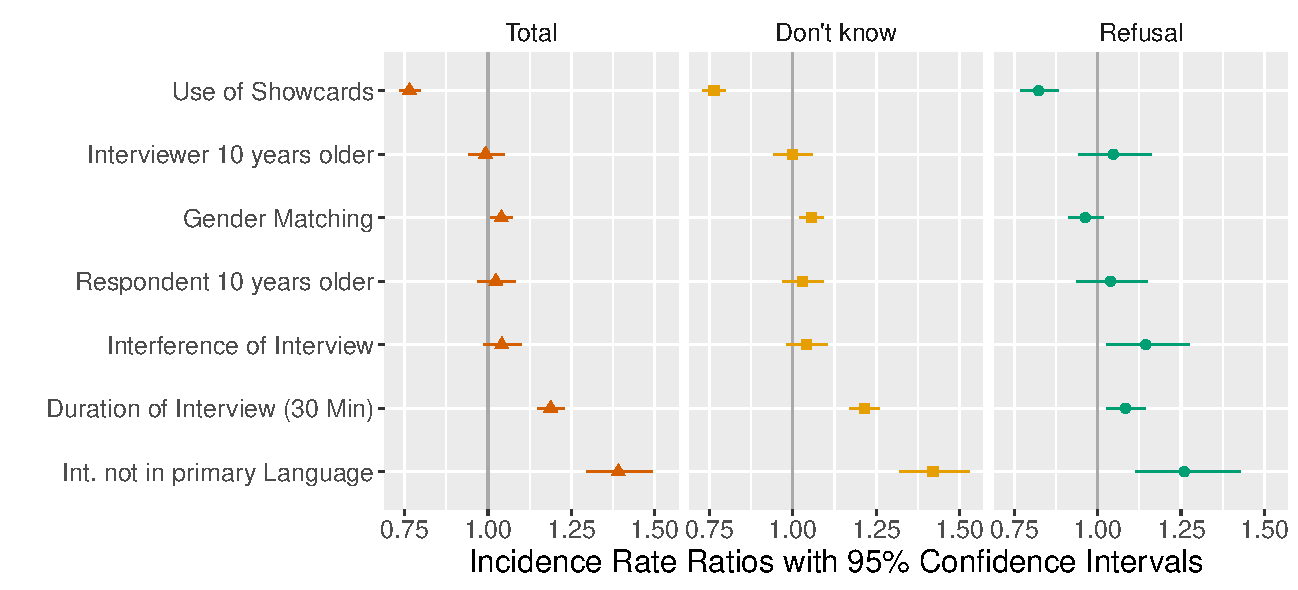
\includegraphics[width=\linewidth]{results_inr_ess9.pdf}
\end{figure}

{\small

\begin{table}[htbp]
   \caption{Regression Results}
   \centering
   \begin{tabular}{lccc}
      \tabularnewline \midrule \midrule
      Dependent Variables:                  & Don't know              & Refusal                 & Total\\  
      Model:                                & (1)                     & (2)                     & (3)\\  
      \midrule
      \emph{Variables}\\
      Number of applicable Items (10 Items) & -0.133$^{***}$          & -0.007                  & -0.112$^{***}$\\   
                                            & (0.010)                 & (0.017)                 & (0.009)\\   
      Interference of Interview             & 0.102$^{***}$           & 0.127$^{*}$             & 0.095$^{***}$\\   
                                            & (0.029)                 & (0.053)                 & (0.027)\\   
      Use of Showcards                      & -0.247$^{***}$          & -0.176$^{***}$          & -0.249$^{***}$\\   
                                            & (0.022)                 & (0.034)                 & (0.020)\\   
      Int. not in primary Language          & 0.389$^{***}$           & 0.256$^{***}$           & 0.366$^{***}$\\   
                                            & (0.038)                 & (0.067)                 & (0.037)\\   
      Gender Matching                       & 0.055$^{**}$            & -0.028                  & 0.042$^{**}$\\   
                                            & (0.017)                 & (0.027)                 & (0.015)\\   
      Respondent 10 years older             & 0.012                   & 0.003                   & 0.003\\   
                                            & (0.030)                 & (0.051)                 & (0.028)\\   
      Interviewer 10 years older            & 0.033                   & 0.038                   & 0.018\\   
                                            & (0.029)                 & (0.051)                 & (0.027)\\   
      Education (ISCED)                     & -0.115$^{***}$          & 0.068$^{***}$           & -0.085$^{***}$\\   
                                            & (0.005)                 & (0.009)                 & (0.005)\\   
      Age                                   & -0.034$^{***}$          & 0.009                   & -0.029$^{***}$\\   
                                            & (0.003)                 & (0.005)                 & (0.003)\\   
      Age squared                           & 0.0004$^{***}$          & $-4.07\times 10^{-5}$   & 0.0003$^{***}$\\   
                                            & ($2.54\times 10^{-5}$)  & ($4.79\times 10^{-5}$)  & ($2.41\times 10^{-5}$)\\    
      Understood Questions                  & -0.348$^{***}$          & -0.052                  & -0.298$^{***}$\\   
                                            & (0.017)                 & (0.027)                 & (0.016)\\   
      Answered to best Ability              & -0.029                  & -0.180$^{***}$          & -0.057$^{***}$\\   
                                            & (0.015)                 & (0.023)                 & (0.014)\\   
      Amount of Clarifications              & 0.254$^{***}$           & 0.598$^{***}$           & 0.330$^{***}$\\   
                                            & (0.011)                 & (0.021)                 & (0.011)\\   
      \midrule
      \emph{Fixed-effects}\\
      Interviewer                           & Yes                     & Yes                     & Yes\\  
      \midrule
      \emph{Fit statistics}\\
      Observations                          & 43,745                  & 36,745                  & 44,000\\  
      Pseudo R$^2$                          & 0.12036                 & 0.18128                 & 0.12289\\  
      Within Pseudo R$^2$                   & 0.05886                 & 0.08776                 & 0.05999\\  
      BIC                                   & 199,301.2               & 92,395.0                & 214,873.6\\  
      Over-dispersion                       & 0.89873                 & 0.75842                 & 1.0379\\  
      \midrule \midrule
      \multicolumn{4}{l}{\emph{Clustered (Interviewer) standard-errors in parentheses}}\\
      \multicolumn{4}{l}{\emph{Signif. Codes: ***: 0.001, **: 0.01, *: 0.05}}\\
   \end{tabular}
\end{table}



}

The most promising ways to reduce item nonresponse seem to be boosting the use of showcards and translating questionnaires. With more frequent showcard use as indicated by the interviewer, the amount of DK reduces by about a quarter and the amount of refusal by about 18\% on average. And compared to interviews conducted in the language the respondent primarily speaks at home, interviews conducted in a language different from the respondents' primary language show on average 42\% more DKs and 26\% more refusals.

As a general observation for all variables, the effects on the total number of item nonresponse closely mirror the effect on DK. This is not surprising since there are many more DKs than refusals. The effects on the number of refusals are typically weaker than the effect on DK but still present. This supports the idea that refusals and DKs are not perfectly separate in their meaning but not identical as well. For the variables presented so far, stronger effects on DK make substantial sense as well since they are all based on respondents' ability or difficulty of the task.

Matching respondents' gender has a small positive effect on the number of DKs. This is contrary to expectations, which suggested that matching the socio-demographics of interviewers and respondents leads to a more trusting interview situation and reduces item nonresponse. The effect on refusals is not significant but should be pronounced since this strategy is partly based on the privacy mechanism. Matching by age has no significant effect. Matching respondents and interviewers seems not to be a promising strategy to reduce item nonresponse.

Other people present during the interview raised the number of refusals by 14\% in line with the reasoning that respondents do not want to answer some questions in the presence of others they know. The effect on DK is not significant. Other people present might therefore influence item nonresponse more via privacy than a distraction. However, due to the relatively small number of refusals, the effect on the total item nonresponse is not significant.

Contrary to expectation, the number of applicable items has a significantly negative effect on DK (and total item nonresponse). A respondent that has been asked 10 questions more has a 12\% lower average number of DK answers.


\section{Discussion}

I have reviewed the literature on item nonresponse and extended the cognitive \textit{satisficing} model \citep{krosnickResponseStrategiesCoping1991} with concerns about privacy to encompass all aspects that can interfere with the response process in survey interviews. Organizing our knowledge into such theoretical models highlights the interrelations between theoretical constructs which is necessary to reduce total error and is not achievable with piece-meal empirical studies. Based on this new model, I have reviewed possibilities to reduce item nonresponse, particularly in face-to-face surveys.

In an empirical analysis using data from the \textit{European Social Survey Round 9}, I found that boosting the respondents' use of showcards and conducting the interview in the respondents' primary language might be promising ways to reduce item nonresponse in face-to-face surveys. These strategies reduce the cognitive effort on behalf of respondents. Other people present during the interview are moderately associated with more refusals. Respondents are probably unwilling to disclose private information in front of people they know. However, my hypothesis that respondents might trust interviewers more and share more information if the interviewer and respondent are socially similar has received no support: matching the socio-demographic characteristics of interviewers and respondents seems not a worthwhile strategy. And surprisingly, longer questionnaires were associated with less item nonresponse. However, this might be related to a problem of operationalization. Most questions that might not apply to respondents are demographics asked at the end. But this would explain no association, but I observe a negative effect for which I do not have an explanation.

Although I carefully selected control variables, I cannot rule out violations of the \textit{conditional independence assumption} which is necessary to identify causal effects with regression analysis. Most variables are influenced by respondents' ability (e.g. to understand survey procedures) as is item nonresponse. Respondents' ability is notoriously hard to measure in surveys and proxies like education and age that I have used as controls are not perfect. A second threat to the results is the endogeneity of some variables of interest, in particular, showcard use and others present during the interviews. They are measured in the interviewer questionnaire after the interview and are likely biased by the interviewers' overall assessment of the interview, including the amount of item nonresponse. I tried to control for that using other variables from the interviewer questionnaire. A third limitation of this analysis concerns the external generalizability of the results. We know that specific types of questions are more prone to item nonresponse, for example, opinions and sensitive questions. The results obtained here reflect the effects on item nonresponse especially on matters of opinion as this is the primary object of study of the ESS. While opinion surveys constitute a large share of surveys and the results should be generalizable to them, other types of surveys might have slightly different challenges concerning item nonresponse.

I nonetheless see value in this analysis for two reasons. First, item nonresponse is relatively rare in single items and therefore difficult to study using survey experiments. Second, and more importantly, the empirical analysis aims to compare multiple potential strategies in their strength of effect (which is not possible using experiments). While it is difficult to assess the true causal effect of the strategies that do make a difference, the strategies that have no effects even in this biased analysis will likely not be successful. This analysis can provide a meaningful starting place for more rigorous tests of the most promising strategies and nonetheless inform survey design choices.

Although I analyze data from a face-to-face survey, I think it is important to anticipate some of the results and especially the implications of the theoretical model for the current shift to self-administrating modes of data collection. The results of my analysis highlight that the most promising strategies to decrease item nonresponse are tools that decrease task difficulty, like showcards and translating questionnaires. In self-administered modes, designing easy-to-use and clear questionnaires and page layouts will be important for item nonresponse. For paper-based modes, this will limit the options for routing and filtering. Specifically, offering refusal and DK as response options is an important design choice. Ethically, respondents need to have the option not to respond. On one hand, this will likely increase item nonresponse. On the other hand, forcing an answer will generate low-quality responses. In self-administered modes, we have less control over the interview situation, for example, whether other people are present. My analysis has shown that the latter is associated with more refusals. The absence of an interviewer reduces social desirability. No social desirability is often considered an advantage as respondents do not need to disclose information to a stranger. But no interviewer could also be a disadvantage as there might be a lower hurdle to satisfice. But the strategies based on the idea that respondents trust socially similar interviewers indicated that the presence of the interviewer might be less important for general levels of item nonresponse. Finally, self-administered modes can be conducted in multiple languages easily because we do not need interviewers that speak a minority language.


\section*{Acknowledgements}

[HIDDEN FOR REVIEW]

%I want to thank Achim Koch, Johanna Mehltretter and especially Tobias Gummer for helpful comments in multiple stages of this project. I want to thank Marcel Kappes and Thomas Gautschi for methodological discussions.

%This work was supported by the University of Mannheim’s Graduate School of Economic and Social Sciences.

\singlespacing
\printbibliography

\end{document}
